%%=============================================================================
%% Methodologie
%%=============================================================================

\chapter{Resultaten van de Praktijktest}
\label{ch:resultaten_praktijk}

Dit onderzoek werd op woensdag 9 mei uitgevoerd door leerkracht Anita Bernard bij 4 testklassen Probleemoplossend Denken 1 in de studierichting Toegepaste Informatica in Gent, België.

\begin{figure}
	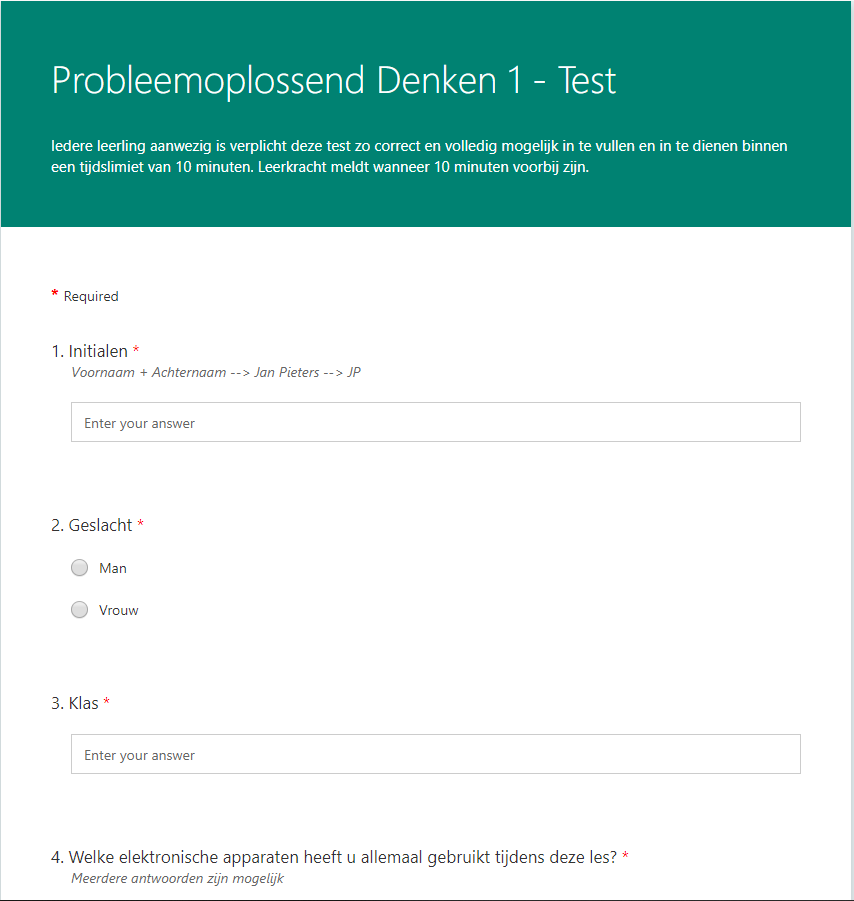
\includegraphics[width=\textwidth]
	{img/vragen-praktijktest.png}
	\caption{Vragen praktijktest voor studenten Toegepaste Informatica }
	\label{fig:vragen-praktijk}
\end{figure}

In figuur \ref{fig:vragen-praktijk} vindt u een screenshot terug van de online test die studenten moesten invullen na de net gegeven theorieles. 

De vragen (met correcte antwoorden) kan u terugvinden in bijlage \ref{ch:qenapraktijk}.

De resultaten van deze test kan u terugvinden via volgende weblink (in Excel-formaat): \url{https://1drv.ms/f/s!AnudQT05fzZSlx83i8B1_PG0OKxa}

Voor men verdergaat, moet men rekening houden met volgende feiten:
\begin{itemize}
	\item Kort is ook overwogen om HBO-ICT uit Nederland hieraan mee te laten doen, maar er is besloten dit niet te doen aangezien zij sinds kort het principe van 'flipped flassrooms' verkiezen. Hierbij moeten studenten in groep één van de lessen van het vak voorbereiden en dan worden de topics die vergeten zijn door de lesgevende studenten aangevuld door de leerkracht. Zo geven ze de leerlingen meer verantwoordelijkheid en wordt de graad van oplettendheid verhoogd. Aangezien er dus een mix is van klasinteractie en pure theorie door de leerkracht, is de opgemaakte test hier niet 100 procent voor geschikt en is besloten de test enkel te doen in België.
	\item In deze test is er spraken van 3 uitschieters (extreme scores). Dit zijn resultaten die volgens de statistiek niet meer in het gekozen betrouwbaarheidsinterval liggen. In dit onderzoek is gekozen voor een betrouwbaarheidsinterval van 95 procent. Dit betekent dat alle scores van de geteste studenten normaal gezien moeten vallen tussen het interval [1,91;8,67]. Deze worden in de test gelaten, aangezien het echt mogelijk is dat een student uitstekend heeft opgelet en zo goed als alle antwoorden juist had. Anderzijds is het ook evengoed mogelijk dat een student totaal geen kennis heeft opgenomen uit een les en bijna elke vraag fout had beantwoord.
	\item In totaal namen 47 studenten deel aan deze test. Dit is niet representatief met de steekproefgrootte die we eerst hadden vooropgesteld voor de bevraging. Deze cijfers mogen hoogstens een goede indicatie zijn over het vak Probleemoplossen Denken 1 aan de Hogeschool Gent. Voor een vergelijking te kunnen maken met andere vakken op de Hogeschool Gent zouden er meerdere klassen moeten getest zijn geweest in verschillende richtingen en vakken.
\end{itemize}

We delen het bekijken van de resultaten op in 3 delen:

\begin{itemize}
	\item In Deel 1 bekijken we de resultaten van alle 47 studenten samen, of ze nu in een controleklas zaten of niet, of ze nu enkel pen en papier mochten gebruiken of veel meer.
	\item In Deel 2 maken we de vergelijking tussen de klassen waarbij alles mocht en de klassen waar er richtlijnen waren.
	\item In Deel 3 kijken we enkel en alleen naar het gedrag van de studenten: hebben ze niets gebruikt of hebben ze gebruik gemaakt van één of ander mobiel apparaat tijdens hun les?
\end{itemize}

\section{DEEL 1: Resultaten van alle studenten}
\label{sec:vragen_res1}

\begin{figure}
	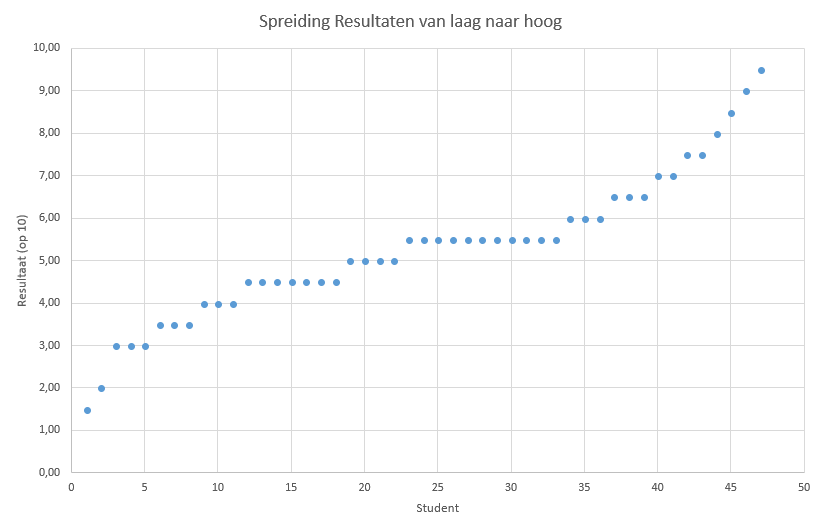
\includegraphics[width=\textwidth]
	{img/spreiding-resultaten.PNG}
	\caption{Spreiding van de resultaten van 47 studenten Toegepaste Informatica}
	\label{fig:spreiding-vragen}
\end{figure}

In totaal namen 47 studenten, verspreid over 4 klassen deel aan dit deelonderzoek. 41 studenten waren van het mannelijk geslacht. Zij scoorden gemiddeld 5,29 op 10, wat beschouwd wordt als zeer nipt geslaagd. Het laagste resultaat liet een man uit Klas 3 opmeten: 1,5 op 10. Het hoogste resultaat mag genoteerd worden door een jongeman uit klas 4: 9,5 op 10. Niemand haalde de perfecte score.

Als we naar de standaardafwijking kijken bij deze studenten, zien we dat eigenlijk 3 resultaten van de 47 geregistreerde waarden buiten het betrouwbaarheidsinterval van 95 procent vallen. 

Enkele opvallende feiten:
\begin{itemize}
	\item Een student kon zelfs toegeven dat hij gebruik maakte van zijn Gameboy Advance SP tijdens de les.
	\item Vraag 1 was de moeilijkste vraag voor de studenten: maar 5 studenten konden hier het goede antwoord geven. Hierin speelt waarschijnlijk mee dat deze een open vraag was.
	\item Vraag 7 werd het best beantwoord door de studenten: 43 van de 47 studenten kruisten het correcte antwoord aan.
\end{itemize}

In Figuur \ref{fig:spreiding-vragen} kan men zien dat de resultaten van de studenten mooi verspreid zijn en er niet echt opvallende uitschieters aanwezig zijn.

\begin{table}[]
	\centering
	\resizebox{\textwidth}{!}{%
		\begin{tabular}{lllll}
			\textbf{Resultaten Alle Studenten}                                                                                          & \textbf{Waarde} &  &  &  \\
			Aantal Studenten                                                                                                            & 47              &  &  &  \\
			Gemiddelde (op 10)                                                                                                          & 5.29            &  &  &  \\
			Mediaan                                                                                                                     & 5.50            &  &  &  \\
			Standaardafwijking                                                                                                          & 1.69            &  &  &  \\
			Aantal studenten die geen devices gebruikten                                                                                & 22              &  &  &  \\
			\begin{tabular}[c]{@{}l@{}}Aantal studenten die wel gebruik maakten\\ van smartphone, laptop of ander apparaat\end{tabular} & 25              &  &  & 
		\end{tabular}%
	}
	\caption{Samenvatting resultaten alle geteste studenten}
	\label{Resultaten_alle_studenten}
\end{table}

Tabel \ref{Resultaten_alle_studenten} geeft enkele cijfers over de test algemeen. Deze tonen aan dat het niet om een gemakkelijke test ging in het algemeen voor de studenten, waarbij de 2 soorten groepen studenten zo goed als gelijk verdeeld zijn.

\section{DEEL 2: Vergelijking tussen de gecontroleerde klassen en de vrije klassen}
\label{sec:vragen_res2}

\begin{table}[]
	\centering
	\resizebox{\textwidth}{!}{%
		\begin{tabular}{l|l|l|l|l|}
			\cline{2-5}
			& \multicolumn{2}{l|}{{ \textbf{CONTROLEKLASSEN}}}                                                                                 & \multicolumn{2}{l|}{{\textbf{VRIJE KLASSEN}}}                                                                                    \\ \hline
			\multicolumn{1}{|l|}{\textbf{Resultaten}}                                                                                                         & \textbf{\begin{tabular}[c]{@{}l@{}}Klas 1\end{tabular}} & \textbf{\begin{tabular}[c]{@{}l@{}}Klas 3\end{tabular}} & \textbf{\begin{tabular}[c]{@{}l@{}}Klas 2\end{tabular}} & \textbf{\begin{tabular}[c]{@{}l@{}}Klas 4\end{tabular}} \\ \hline
			\multicolumn{1}{|l|}{Aantal Studenten}                                                                                                            & 10                                                               & 11                                                               & 14                                                               & 12                                                                \\ \hline
			\multicolumn{1}{|l|}{Gemiddelde (op 10)}                                                                                                          & 5.40                                                             & 5.77                                                             & 4.57                                                             & 5.58                                                              \\ \hline
			\multicolumn{1}{|l|}{Mediaan}                                                                                                                     & 5.50                                                             & 5.50                                                             & 4.50                                                             & 5.50                                                              \\ \hline
			\multicolumn{1}{|l|}{Standaardafwijking}                                                                                                          & 1.35                                                             & 2.00                                                             & 1.25                                                             & 1.99                                                              \\ \hline
			\multicolumn{1}{|l|}{Aantal studenten die geen devices gebruikten}                                                                                & 8                                                                & 11                                                               & 0                                                                & 3                                                                 \\ \hline
			\multicolumn{1}{|l|}{\begin{tabular}[c]{@{}l@{}}Aantal studenten die wel gebruik maakten\\ van smartphone, laptop of ander apparaat\end{tabular}} & 2                                                                & 0                                                                & 14                                                               & 9                                                                 \\ \hline
		\end{tabular}%
	}
	\caption{Samenvatting resultaten klassen}
	\label{resultaten_klassen}
\end{table}

\begin{figure}
	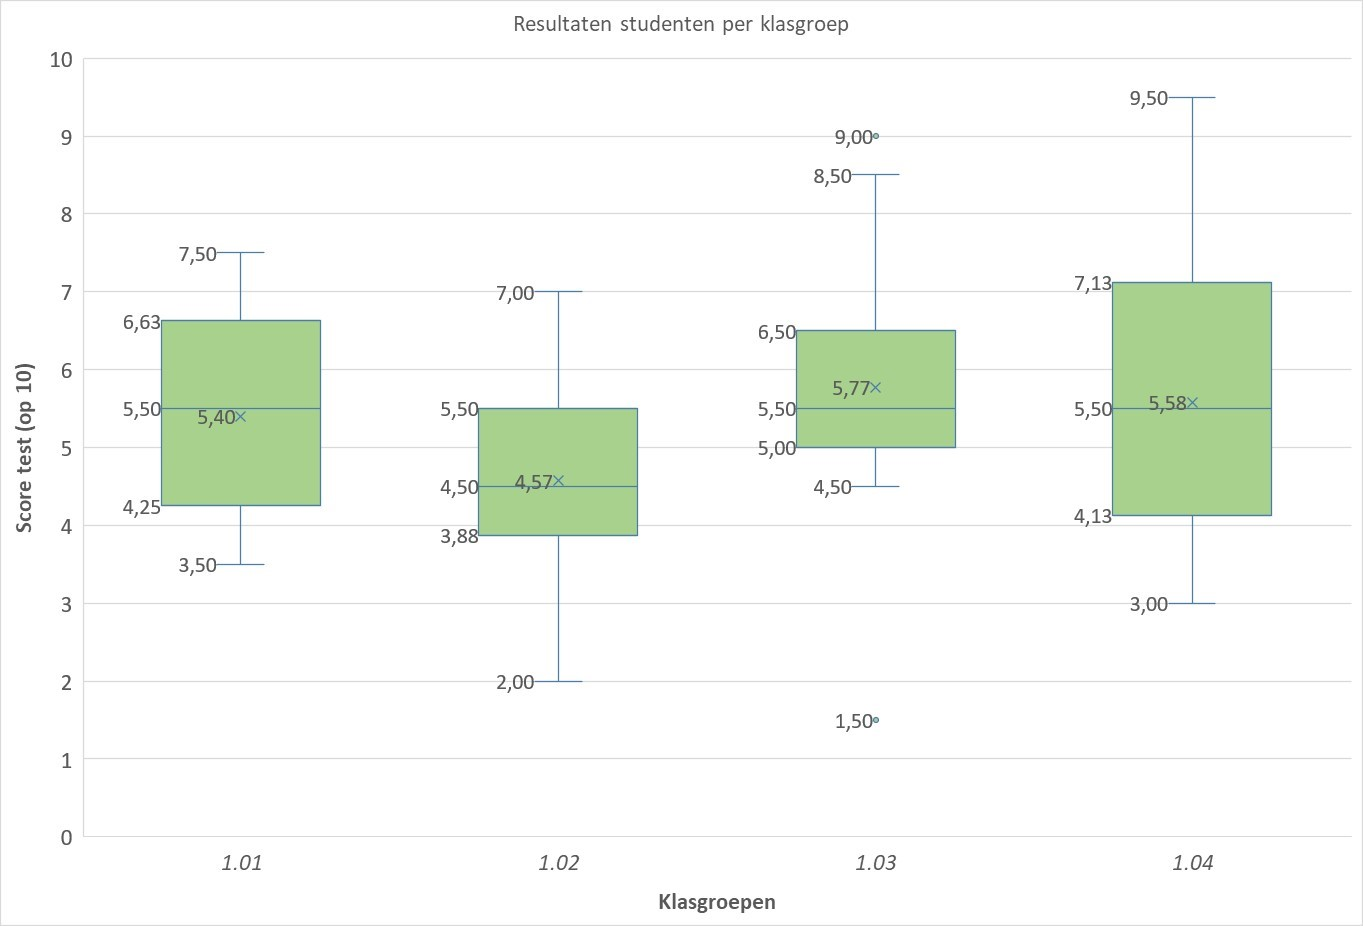
\includegraphics[width=\textwidth]
	{img/Boxplot3.jpg}
	\caption{Spreiding van alle klassen afzonderlijk}
	\label{fig:boxplot3}
\end{figure}

In dit deel bekijken we de verschillen tussen de klassen onderling. De eerste en derde klas die mevrouw Bernard les gaf (Klas 1 en Klas 3) waren onderhevig aan de strenge regels die het onderzoek hadden vooropgesteld: geen kans tot afleiding van smartphone en laptop en enkel en alleen gebruik makend van pen en papier. Klas 2 en Klas 4 waren, als dezelfde redenering gevolgd wordt als in de vorige zin, vrije klassen: studenten uit deze klassen werden niet tegengehouden om gebruik te maken van een elektronisch device om deze les te volgen. In Tabel \ref{resultaten_klassen} kan u de verschillen zien tussen de geteste klassen.

Klas 3, waar niemand valsspeelde en waar iedereen de richtlijnen van de leerkracht volgde, had de beste resultaten: met een gemiddelde van 5,77 op 10 zijn zij de beste klas. Zij konden tijdens de les het meeste oppikken en onthouden.

Klas 2, waar iedereen gebruik maakte van een laptop en/of smartphone en mogelijks afgeleid werden door sociale media, berichten en grappige filmpjes, scoorde het slechtst. Zowel het gemiddelde als de mediaan van deze klas zijn onder de grens van 5 op 10.

Tussen de slechtste klas en de beste klas kunnen we dus een verschil van 1,2 punten op 10 opmeten, ofwel 12 procent. Het kan natuurlijk zijn dat klas 2 minder begaafde studenten bevat en klas 3 slimme studenten, maar het verschil van 12 procent kan toch niet volledig hieraan te wijden zijn.

Vervolgens kijken we verder en we groeperen de controleklassen tot 1 klas en de vrije klassen tot 1 klas. Het gemiddelde van de controleklassen is 5,60 op 10, waar het resultaat van de 2 vrije klassen samen gemiddeld 5,04 op 10 is. Hier meten we dus een verschil van 5,6 procent tussen beide soorten klassen.

Figuur \ref{fig:boxplot3} geeft een beeld van de uitschieters en interkwartielafstanden voor elke klas. De afstanden tussen het 1ste kwartiel en het minimum zijn bij de controleklassen (klassen 1.01 en 1.03) zeer beperkt, waar bij de vrije klassen deze afstand groter is. Dit toont aan dat de studenten met normaal lage punten in de controleklassen door de maatregel ook beter gescoord hebben. 


\section{DEEL 3: Vergelijking tussen studenten met pen en papier en studenten met elektronische hulpmiddelen}
\label{sec:vragen_res3}

In het laatste deel vergeten we de opdeling van studenten in klassen en maken we een vergelijking tussen de student die geen gebruik maakt van laptop, smartphone of Gameboy tijdens de les en de student die wel gebruik maakt van deze hedendaagse snufjes. De vergelijking tussen deze twee soorten studenten vindt u terug in tabel \ref{resultaten_studenten}. 

\begin{table}[]
	\centering
	\resizebox{\textwidth}{!}{%
		\begin{tabular}{|l|l|l|}
			\hline
			\textbf{Resultaten Soorten Student} & \textbf{\begin{tabular}[c]{@{}l@{}}Student met\\ pen en papier\end{tabular}} & \textbf{\begin{tabular}[c]{@{}l@{}}Student met\\ elektronica\end{tabular}} \\ \hline
			Aantal Studenten                    & 22                                                                    & 25                                                                    \\ \hline
			Gemiddelde (op 10)                  & 5.73                                                                  & 4.90                                                                  \\ \hline
			Mediaan                             & 5.50                                                                  & 4.50                                                                  \\ \hline
			Standaardafwijking                  & 1.70                                                                  & 1.62                                                                  \\ \hline
		\end{tabular}%
	}
	\caption{Samenvatting resultaten soort student}
	\label{resultaten_studenten}
\end{table}

De student die dus genoodzaakt is om de hele les naar ofwel buiten, naar het bord of naar de leerkracht te kijken, scoort gemiddeld dus 8,3 procent beter dan een student die ook nog de keuze heeft genomen om zijn smartphone of laptop te gebruiken tijdens de les. De hogere standaardafwijking bij de klassieke student duidt op een grotere verspreiding van de scores binnen die groep. 


De cijfers tonen het duidelijk aan: mensen die gebruik maken van laptops en smartphones tijdens een theoretische les zullen het klaslokaal uitstappen met minder kennis over de les dan de student die sterk genoeg was om zijn smartphone of laptop in zijn rugzak te laten zitten. Hoe sterk dit negatief effect is, valt niet met 100 procent zekerheid af te leiden uit deze kleine test met kleine steekproefgrootte. Aan de hand van deze metingen kunnen we wel inschatten dat voor studenten die het vak Probleemoplossend Denken 1 hebben in de studierichting Toegepaste Informatica dit negatief effect schommelt tussen de 5 à 10 procent.



